% ltex: language=it
\chapter{Linguaggi Liberi dal Contesto}\label{chap:ll_linguaggi_liberi_dal_contesto} % (fold)
Visto che molti linguaggi non sono \hyperref[def:ling-reg]{Regolari}, allora è necessario considerare una classe più estesa dei linguaggi:
\begin{itemize}
    \item \ac{cfl}, \textit{linguaggi liberi dal contesto}, usati nello studio dei \hyperref[sec:i_linguaggi_naturali]{Linguaggi Naturali} dal 1950;
    \item \ac{cfg}, \textit{grammatiche libere dal contesto}, sono la base della sintassi \ac{bnf}, usate per i linguaggi di programmazione;
\end{itemize}
%
\section{Grammatiche Libere dal Contesto}\label{sec:ll_grammatiche_libere_dal_contesto} % (fold)
\begin{example}{Esempio Informale di CFG}{}
    \begin{definition}{Palindromo}{palindromo}
        Una stringa $w$ è \textbf{palindroma} se e solo se:
        \[
            w = w^R
        \]
    \end{definition}
    Si considera il \hyperref[def:ling-reg]{Linguaggio Regolare} dei \textit{palindromi} $L_{pal} = \pg{w\in\Si[*]:w = w^R}$, sia $\Si = \pg{0,1}$.
    Sia $n$ il numero di stati di un ipotetico \hyperref[sub:lr_dfa]{DFA} $A$ tale che $L(A) = L_{pal}$.
    Si ha che
    \[
        0^n10^n \in L_{pal}
    \]
    \begin{note}[Contraddizione]
        Nel leggere lo $0^n$ iniziale $A$ deve passere per un \textbf{loop}.
        Se omettiamo il loop, $A$ accetta una stringa $0^m10^n$ con $m < n$.
    \end{note}
    Si definisce $L_{pal}$ induttivamente:
    \begin{description}
        \item[Base] $\eps$, $0$ e $1$ sono \hyperref[def:palindromo]{Palindromi}.
        \item[Induzione] Se $w$ è una \hyperref[def:palindromo]{Palindrome}, anche $0w0$ e $1w1$ lo sono.
    \end{description}
\end{example}
Le \ac{cfg}, invece, sono un modo \textbf{formale} per definizione come quella per $L_{pal}$:
\[
    \begin{aligned}
        & 1.\quad S \to \eps \\
        & 2.\quad S \to 0 \\
        & 3.\quad S \to 1 \\
        & 4.\quad S \to 0S0 \\
        & 5.\quad S \to 1S1 \\
    \end{aligned}
\]
\begin{itemize}
    \item $0$ e $1$ sono \textbf{terminali};
    \item $S$ è una \textbf{categoria sintattica}, o più tecnicamente \textbf{variabile};
    \item $S$ è in questa grammatica anche la categoria sintattica \textit{iniziale};
    \item $1-5$ sono \textbf{produzioni} o \textbf{regole};
\end{itemize}
\begin{definition}{Grammatica Libera dal Contesto}{cfg}
    Una \textbf{grammatica libera dal contesto} è una quadrupla:
    \[
        G = \pt{V,T,P,S}
    \]
    dove:
    \begin{itemize}
        \item $V$ è un insieme finito di simboli che formano le stringhe del linguaggio da definire (\textbf{terminali} o \textbf{simboli terminali});
        \item $T$ è un insieme finito di \textbf{variabili}: ogni variabile rappresenta un linguaggio, ossia un insieme di stringhe;
        \item $P$ è un insieme finito di \textbf{produzioni} o \textbf{regole}, che rappresentano la definizione ricorsiva del linguaggio.
            Ogni produzione consiste di tre parti:
            \begin{itemize}
                \item una variabile definita (parzialmente) dalla produzione ed è spesso detta la \textbf{testa} della produzione;
                \item il simbolo di produzione $\to$
                \item una stringa di zero o più terminali e variabili, detta il \textbf{corpo della produzione}: rappresenta un modo di formare le stringhe nel linguaggio della variabile di testa;
            \end{itemize}
        \item $S$ è una variabile, chiamata \textbf{simbolo iniziale} o \textbf{variabile iniziale}, che rappresenta il linguaggio da definire;
    \end{itemize}
\end{definition}
\begin{example}{}{}
    La grammatica $G_{pal}$ per le palindrome è rappresentata da:
    \[
        G_{pal} = \pt{\pg{S},\pg{0,1},P,S}
    \]
    dove $P = \pg{S\to\eps,S\to0,S\to1,S\to0S0,S\to1S1}$
    \begin{note}[A volte si raggruppano le produzioni con la stessa testa]
        \[
            \pg{S \to \eps|0|1|0S0|1S1}
        \]
    \end{note}
\end{example}
\begin{example}{Espressioni di un tipico linguaggio di programmazione}{}
    Gli operatori sono $+$ e $*$, e gli operandi sono identificatori, cioè stringhe in
    \[
        L\pt{\pt{a+b}(a+b+0+1)^*}
    \]
    Le espressioni sono definite dalla grammatica:
    \[
        G = \pt{\pg{E,I},T,P,E}
    \]
    dove $T = \pg{+,*,(,),a,b,0,1}$ e $P$ è il seguente insieme di produzioni:
    \[
        \begin{aligned}
            1.\quad E &\to I \\
            2.\quad E &\to E+E\\
            3.\quad E &\to E*E\\
            4.\quad E &\to (E)\\
            5.\quad I &\to a\\
            6.\quad I &\to b\\
            7.\quad I &\to Ia\\
            8.\quad I &\to Ib\\
            9.\quad I &\to I0\\
            10.\quad I &\to I1\\
        \end{aligned}
    \]
\end{example}
%
% section Grammatiche Libere dal Contesto (end)
\section{Derivazioni per mezzo di una Grammatica}\label{sec:ll_derivazioni_per_mezzo_di_una_grammatica} % (fold)
Le \textbf{produzioni} di una \hyperref[def:cfg]{CFG} si applicano per dedurre che determinate stringhe appartengono al linguaggio di una certa variabile.
La deduzione può seguire due strade:
\begin{description}
    \item[Inferenza Ricorsiva] Si serve delle regole utilizzando il corpo per passare alla testa.
        Ovvero si prendono stringhe di cui si conoscono l'appartenenza al linguaggio di ognuna delle variabili del corpo, si concatenano nell'ordine adeguato con i termini che compaiono nel corpo e si deduce che la stringa risultante è nel linguaggio della variabile che compare in testa. 
    \item[Derivazione] Si applicano le \textbf{produzioni} dalla testa al corpo.
        Si espande il simbolo iniziale usando una delle sue produzioni, cioè usando una produzione la cui testa sia il simbolo iniziale.
        Successivamente si espande nuovamente la stringa risultante sostituendo una delle variabili con il corpo di una delle sue produzioni, e così via, fino a derivare una stringa fatta interamente di \textbf{terminali}.
        \begin{note}
            Il linguaggio della grammatica è l'insieme di tutte le stringhe di terminali ottenute con questa procedura
        \end{note}
\end{description}
\begin{remark}{Derivazione}{gram-derivazione}
    Si definisce $\overset{*}{\implies}$ la \textbf{chiusura riflessiva} e \textbf{transitiva} dell'operatore $\implies$.
    \begin{description}
        \item[Base] Per qualsiasi stringa $\al$ di terminali e variabili, $\al\overset{*}{\implies}\al$, in altri termini qualunque stringa deriva se stessa
        \item[Induzione] Se $\al\overset{*}{\implies}\bt$ e $\bt\overset{*}{\implies}\gm$, allora $\al\overset{*}{\implies}\gm$.
            Ossia se $\al$ può diventare $\beta$ in zero o più passi, e un passo ulteriore trasforma $\beta$ in $\gm$, allora $\alpha$ può diventare $\gamma$.
            \\
            Detto in altri termini, $\alpha\overset{*}{\implies}\beta$ significa che esiste una sequenza di stringhe $\vc{\gm_1}{\gm_n}$ con $n\ge1$ tale che:
            \begin{enumerate}
                \item $al = \gm_1$
                \item $\beta = \gm_n$
                \item per $\for[][][n-1]$ abbiamo $\gm_i \implies \gm_{\inc i}$
            \end{enumerate}
    \end{description}
\end{remark}
\begin{example}{Derivazione di una stringa nella grammatica delle espressioni}{}
    Data la stringa $a*(a+b00)$ si può derivare $E$ in questo modo:
    \[
        \begin{aligned}
            &E \imp E*E\imp I*E\imp a*E\imp a*(E)\imp a*(E+E)\imp \\
            &a*(I+E)\imp a*(a+E)\imp a*(a+I)\imp a*(a+I0)\imp \\
            &a*(a+I00)\imp a*(a+b00)
        \end{aligned}
    \]
    \begin{note}
        A ogni passo potremmo avere varie regole tra cui scegliere, ad esempio:
        \[
            \begin{aligned}
                &I*E\imp a*E\imp a*(E) \text{ oppure} \\
                &I*E\imp I*(E)\imp a*(E)
            \end{aligned}
        \]
        \begin{critical}[Non tutte le scelte portano a derivazioni di una particolare stringa]
            Ad esempio non è possibile derivare $a*(a+b00)$ utilizzando:
            \[
                E\imp E+E
            \]
        \end{critical}
    \end{note}
\end{example}
\subsection{Derivazioni a Sinistra e a Destra}\label{sub:ll_derivazioni_a_sinistra_e_a_destra} % (fold)
\begin{description}
    \item[Derivazione a Sinistra $\underset{lm}{\imp}$] Rimpiazza sempre la variabile più a sinistra con il corpo di una delle sue regole.
    \item[Derivazione a Destra $\underset{rm}{\imp}$] Rimpiazza sempre la variabile più a destra con il corpo di una delle sue regole.
\end{description}
\begin{example}{Derivazione a Destra}{}
    \[
        \begin{aligned}
            E &\underset{rm}{\implies}E*E \underset{rm}{\implies} E*(E) \underset{rm}{\implies} E*(E+E) \underset{rm}{\implies} E*(E+I) \\
            &\underset{rm}{\implies}E*(E+I0) \underset{rm}{\implies}E*(E+I00) \underset{rm}{\implies}E*(E+b00) \\
            &\underset{rm}{\implies} E*(I+b00) \underset{rm}{\implies}E*(a+b00) \underset{rm}{\implies}I * (a+b00) \underset{rm}{\implies} a * (a+b00)
        \end{aligned}
    \]
\end{example}
% subsection Derivazioni a Sinistra e a Destra (end)
%
\subsection{Il Linguaggio della Grammatica}\label{sub:ll_il_linguaggio_della_grammatica} % (fold)
Se $G=\pt{V,T,P,S}$ è un \hyperref[def:cfg]{CFG}, allora il \textbf{linguaggio} di $G$ è
\[
    L(G) = \pg{w\in T^*:S \overset{*}{\implies}w}
\]
\begin{note}
    Cioè l'insieme delle stringhe su $T^*$ \hyperref[rem:gram-derivazione]{Derivabili} dal simbolo iniziale.
\end{note}
% subsection Il Linguaggio della Grammatica (end)
% section Derivazioni per mezzo di una Grammatica (end)
%
\section{Alberi Sintattici}\label{sec:ll_alberi_sintattici} % (fold)
\begin{definition}{Albero Sintattico}{alb-sint}
    Un \textbf{albero sintattico} mostra in modo chiaro come i simboli di una stringa terminale sono raccolti in sottostringhe, ciascuno appartenente al linguaggio di una delle variabili della grammatica.
    \begin{note}
        Se $w \in L(G)$, per una \hyperref[def:cfg]{CFG}, allora $w$ ha un \textit{albero sintattico} che rappresenta la \textbf{struttura sintattica} di $w$.
        \begin{tip}
            Gli alberi sintattici sono una \textbf{rappresentazione alternativa delle derivazioni}
        \end{tip}
    \end{note}
    \begin{critical}[Non esiste un solo albero sintattico per un linguaggio]
    \end{critical}
\end{definition}
%
\subsection{Costruzione di Alberi Sintattici}\label{sub:ll_costruzione_di_alberi_sintattici} % (fold)
Fissata una grammatica $G = (V,T,P,S)$, gli \textbf{alberi sintattici} di $G$ sono alberi che soddisfano le seguenti condizioni:
\begin{enumerate}
    \item ciascun \textbf{nodo interno} è etichettato da una \textbf{variabile} $V$;
    \item ciascuna \textbf{foglia} è etichettata da una \textbf{variabile} (simbolo in $V\cup T\cup\pg\eps$);
        \begin{note}
            Se una foglia è etichettata con $\eps$, deve essere l'unico figlio del suo genitore
        \end{note}
    \item Se un \textbf{nodo interno} è etichettato $A$, e i suoi figli, a partire da sinistra, sono \textbf{etichettati}: siano $\vc{X_1}{X_2}$ allora $A$ è una \textbf{produzione} in $P$
        \[
            A \to \vc{X_1}{X_2} \in P
        \]
        \begin{note}
            Un $X$ può essere $\epsilon$ solo nel caso in cui è l'\textbf{etichetta} di un figlio unico, e quindi $A\to\eps$ è una produzione di $G$
        \end{note}
\end{enumerate}
\begin{example}{}{}
    La grammatica:
    \[
        \begin{aligned}
            1.\quad E &\to I \\
            2.\quad E &\to E+E\\
            3.\quad E &\to E*E\\
            4.\quad E &\to (E)\\
                      &\vdots
        \end{aligned}
    \]
    può essere rappresentata nel seguente albero sintattico
    \begin{cimage}
        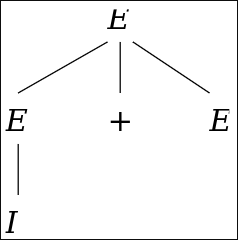
\includegraphics[width=.4\textwidth]{assets/20261015_120304.png}
        \caption{Si mostra la derivazione $E \overset{*}{\implies}I+E$}
    \end{cimage}
    \begin{note}
        La radice è etichettata dalla variabile$E$.
        \\
        La produzione applicata alla radice è $E\to E+E$: i tre figli della radice hanno, a partire da sinistra, le etichette $E$, $+$ e $E$.
        \\
        Per il figlio più a sinistra della radice si applica la produzione $E\to I$: il nodo ha un solo figlio, etichettato $I$.
    \end{note}
\end{example}
% subsection Costruzione di Alberi Sintattici (end)
%
\subsection{Prodotto di un Albero Sintattico}\label{sub:ll_prodotto_di_un_albero_sintattico} % (fold)
\begin{definition}{Prodotto}{alb-prodotto}
    Il \textbf{prodotto} di un albero sintattico è la \textbf{stringa di foglie da sinistra a destra} concatenate fra loro
    \begin{note}[È sempre una stringa derivata dalla variabile della radice]
    \end{note}
\end{definition}
Di particolare importanza sono gli alberi sintattici che soddisfano queste condizioni:
\begin{itemize}
    \item il \hyperref[def:alb-prodotto]{Prodotto} è una \textbf{stringa terminale}, in questo caso tutte le foglie sono etichettate da un \textbf{terminale} o da $\eps$;
    \item la radice è etichettata dal \textbf{simbolo iniziale};
\end{itemize}
\begin{note}
    L'insieme di prodotti di questi \hyperref[def:alb-sint]{Alberi Sintattici} rappresenta \hyperref[sub:ll_il_linguaggio_di_una_grammatica]{Il Linguaggio della Grammatica}
\end{note}
\begin{example}{}{}
    \begin{cimage}
        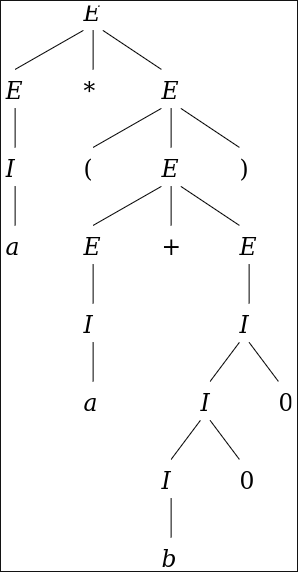
\includegraphics[width=.2\textwidth]{assets/20261015_122710.png}
    \end{cimage}
    Il prodotto è pari a: $a*(a*b00)$
\end{example}
%
\paragraph{Inferenza, Derivazioni e Alberi Sintattici}\label{par:ll_inferenza_derivazioni_e_alberi_sintattici} % (fold)
Data una \hyperref[def:cfg]{Grammatica} $G=(V,T,P,S)$, e $A\in V$, i seguenti enunciati sono equivalenti:
\begin{itemize}
    \item[$\to$] la procedura di \textbf{inferenza ricorsiva} stabilisce che la stringa terminale $w$ è nel linguaggio della variabile $A$;
    \item $A\overset{*}{\implies}w$
    \item $A\overset{*}{\underset{lm}{\implies}}w$ e $A\overset{*}{\underset{rm}{\implies}}w$
    \item esiste un albero sintattico $G$ con radice $A$ e prodotto $w$;
\end{itemize}
\begin{note}
    Se escludiamo l'inferenza ricorsiva, definita solo per stringhe terminali, le altre condizioni --- l'esistenza di derivazioni generiche, a sinistra o a destra, e di alberi sintattici --- sono \textbf{equivalenti} anche se $w$ contiene \textbf{variabili}
\end{note}
\begin{warning}[Dimostrazioni]
    Per provare l'equivalenza si procede seguendo il seguente piano:
    \begin{itemize}
        \item dagli alberi alle derivazioni a sinistra (destra): visto l'albero da sinistra a destra (da destra a sinistra);
        \item una derivazione sinistra (o destra) è anche una derivazione;
        \item leggendo la derivazione costruisco l'albero;
    \end{itemize}
\end{warning}
\begin{cimage}
    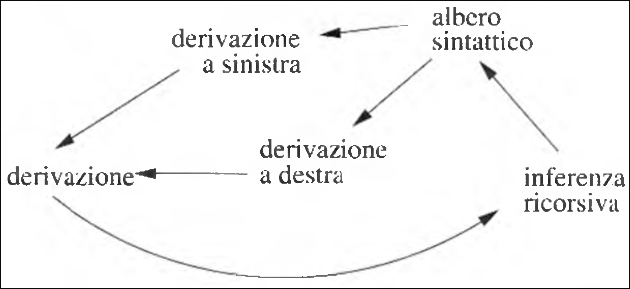
\includegraphics[width=.4\textwidth]{assets/20261015_123514.png}
    \caption{Derivazione dell'equivalenza di alcuni enunciati}\label{fig:20261015_123514}
\end{cimage}
\begin{example}{Costruire la derivazione a sinistra di un albero}{}
    Dato il seguente \hyperref[def:alb-sint]{Albero Sintattico}
    \begin{cimage}
        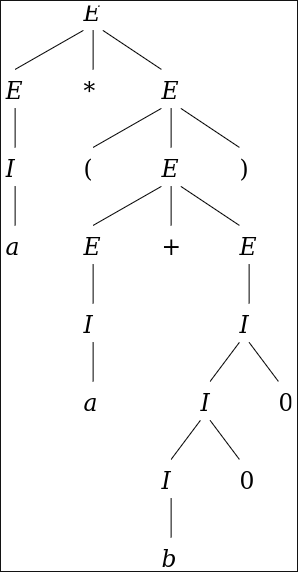
\includegraphics[width=.3\textwidth]{assets/20261015_122710.png}
    \end{cimage}
    Prendendo tutti i sottoalberi della radice (sinistra $E\to I\to a$ e destra $E\to E^*\to +^*$):
    \begin{description}
        \item[Sinistra] Si suppone di aver costruito induttivamente l'albero in questo modo:
            \[
                E \underset{lm}{\implies}I \underset{lm}{\implies}a
            \]
        \item[Destra] Si suppone di aver costruito induttivamente l'albero in questo modo:
            \[
                \begin{aligned}
                    &E \underset{lm}{\implies}(E) \underset{lm}{\implies}(E+E) \underset{lm}{\implies}(I+E) \underset{lm}{\implies}(a+E)\underset{lm}{\implies} \\
                    &(a+I)\underset{lm}{\implies}(a+I0)\underset{lm}{\implies}(a+I00)\underset{lm}{\implies}(a+b00)
                \end{aligned}
            \]
    \end{description}
    Per la derivazione corrispondente all'intero albero, iniziamo con $E \underset{lm}{\implies}E*E$ e si espande la prima $E$ (perché si deriva a sinistra in questo caso) con la prima derivazione e la seconda $E$ con la seconda derivazione:
    \[
        \begin{aligned}
            &E \underset{lm}{\implies}E*E \\
            &\underset{lm}{\implies} I*E \\
            &\underset{lm}{\implies}a*E \\
            &\underset{lm}{\implies}a*(E) \\
            &\underset{lm}{\implies}a*(E+E) \\
            &\underset{lm}{\implies}a*(I+E) \\
            &\underset{lm}{\implies}a*(a+E) \\
            &\underset{lm}{\implies}a*(a+I) \\
            &\underset{lm}{\implies}a*(a+I0) \\
            &\underset{lm}{\implies}a*(a+I00) \\
            &\underset{lm}{\implies}a*(a+b00) \\
        \end{aligned}
    \]
\end{example}
% paragraph Inferenza, Derivazioni e Alberi Sintattici (end)
% subsection Prodotto di un Albero Sintattico (end)
% section Alberi Sintattici (end)
%
\section{Ambiguità nelle Grammatiche e nei Linguaggi}\label{sec:ll_ambiguit_nelle_grammatiche_e_nei_linguaggi} % (fold)
Nella grammatica:
\[
    \begin{aligned}
        1.\quad E &\to I \\
        2.\quad E &\to E+E \\
        3.\quad E &\to E*E \\
        4.\quad E &\to (E) \\
        &\vdots
    \end{aligned}
\]
$E+E*E$ ha due derivazioni:
\begin{multicols}{2}
    \begin{itemize}
        \item $E\imp E+E\imp E+E*E$
        \item $E\imp E*E\imp E+E*E$
    \end{itemize}
\end{multicols}
Questo ci dà due alberi sintattici:
\begin{cimage}
    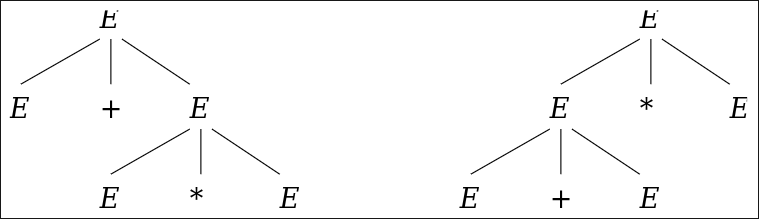
\includegraphics[width=.6\textwidth]{assets/20261015_132527.png}
\end{cimage}
\begin{warning}[L'esistenza di varie \textit{derivazioni} di per se non è pericolosa, ma l'esistenza di vari alberi sintattici \textit{rovina} la {\hyperref[def:cfg]{Grammatica}}]
\end{warning}
\begin{definition}{Ambiguità}{ambiguita}
    Sia $G=(V,T,P,S)$ una \hyperref[def:cfg]{CFG}, diciamo che $G$ è \textbf{ambigua} se esiste una stringa in $T^*$ che ha più di un \hyperref[def:alb-sint]{Albero Sintattico}.
    \emptyln{}
    Se ogni stringa in $L(G)$ ha un \textit{unico} \hyperref[def:alb-sint]{Albero Sintattico}, $G$ è detta \textbf{non ambigua}.
\end{definition}
\begin{example}{}{}
    La stringa terminale $a+a*a$ ha due alberi sintattici:
    \begin{cimage}
        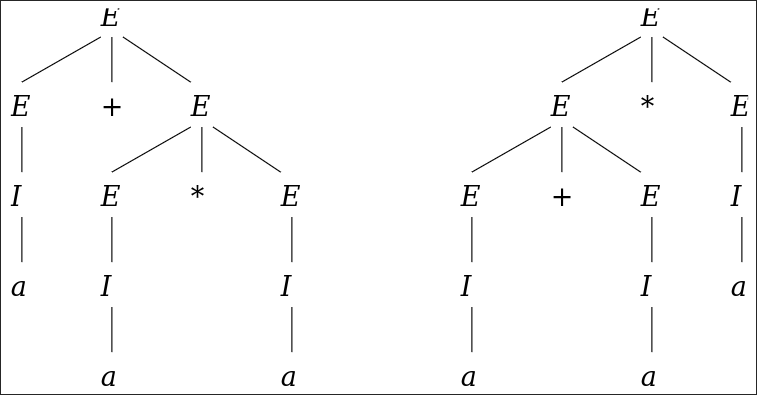
\includegraphics[width=.6\textwidth]{assets/20261015_133845.png}
    \end{cimage}
\end{example}
\begin{note}[In generale]
    \begin{itemize}
        \item A un \hyperref[def:alb-sint]{Albero Sintattico} corrispondono molte \hyperref[rem:gram-derivazione]{Derivazioni};
        \item A ogni diverso \hyperref[def:alb-sint]{Albero Sintattico} corrisponde un'unica diversa \hyperref[rem:gram-derivazione]{Derivazione} a sinistra;
        \item A ogni diverso \hyperref[def:alb-sint]{Albero Sintattico} corrisponde un'unica diversa \hyperref[rem:gram-derivazione]{Derivazione} a destra;
    \end{itemize}
\end{note}
\begin{theorem}{}{}
    Data una \hyperref[acro:cfg]{CFG} $G$, una \textbf{stringa terminale} $w$ ha due distinti \hyperref[def:alb-sint]{Alberi Sintattici} se e solo se $w$ ha due distinte \hyperref[rem:gram-derivazione]{Derivazioni} a sinistra dal \textbf{simbolo iniziale}
\end{theorem}
%
\subsection{Rimuovere l'Ambiguità dalle Grammatiche}\label{sub:ll_rimuovere_l_ambiguit_dalle_grammatiche} % (fold)
Non è esiste un algoritmo specifico per poter riconoscere le ambiguità e oltretutto non è sempre possibile rimuoverle.
\begin{example}{}{}
    Data la grammatica:
    \[
        \begin{aligned}
            &E\to I|E+E|E*E|(E) \\
            &I\to a|b|Ia|Ib|I0|I1
        \end{aligned}
    \]
    si vuole modificarla in maniera tale da stabilire:
    \begin{itemize}
        \item la precedenza tra $*$ e $+$;
        \item il raggruppamento di sequenze di uno stesso stato operatore: $E+E+E$ è inteso come $E+(E+E)$ oppure come $(E+E)+E$?
    \end{itemize}
\end{example}
Per risolvere il problema dell'esempio precedente, si introduce una \textbf{gerarchia di variabili} che stabilisca un ordine di precedenza tra gli operatori:
\begin{enumerate}
    \item \textit{espressioni} $E$: composizioni di uno o più \textit{termini} $T$ tramite $+$
    \item \textit{termini} $T$: composizioni di uno o più \textit{fattori} $F$ tramite $*$
    \item \textit{fattori} $F$: \textit{identificatori} $I$ ed \textit{espressioni} $E$ racchiuse tra parentesi
\end{enumerate}
\begin{note}
    I termini $T$ non possono generare $+$ che siano fuori da parentesi: questa gerarchia stabilisce che $*$ \textbf{ha precedenza rispetto a} $+$
\end{note}
Ad esempio l'unico modo di generare $a+a*a$ è considerando $a*a$ come un termine $T$, formalmente:
\[
    \begin{aligned}
        1.\ E&\to T|E+E \\
        2.\ T&\to F|T*T \\
        3.\ F&\to I|(E) \\
        4.\ I&\to a|b|Ia|Ib|I0|I1
    \end{aligned}
\]
\begin{note}[Questa grammatica è \textit{non ambigua}?]
    No, bisogna anche imporre un ordine per raggruppamento degli operatori allo stesso livello
\end{note}
Quindi la grammatica diventa:
\[
    \begin{aligned}
        1.\ E&\to T|E+T \\
        2.\ T&\to F|T*F \\
        3.\ F&\to I|(E) \\
        4.\ I&\to a|b|Ia|Ib|I0|I1
    \end{aligned}
\]
e come unico \hyperref[def:alb-sint]{Albero Sintattico} non ambiguo si ottiene:
\begin{cimage}
    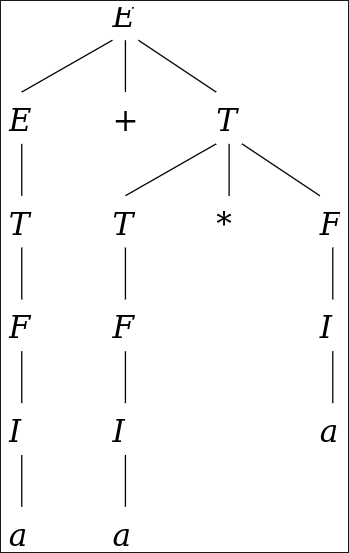
\includegraphics[width=.4\textwidth]{assets/20261015_162029.png}
\end{cimage}
% subsection Rimuovere l'Ambiguità dalle Grammatiche (end)
%
\subsection{Ambiguità Inerente}\label{sub:ll_ambiguit_inerente} % (fold)
\begin{definition}{Inerentemente Ambiguo}{ambig-inerente}
    Un \ac{cfl} $L$ è \textbf{inerentemente ambiguo} se tutte le grammatiche per $L$ sono ambigue
\end{definition}
\begin{example}{}{}
    Considerando:
    \[
        L = \pg{a^nb^nc^md^m:n\ge 1,m\ge 1}\cup\pg{a^nb^mc^md^n:n\ge 1, m\ge 1}
    \]
    una possibile \hyperref[def:cfg]{Grammatica} per $L$ è:
    \[
        \begin{aligned}
            S &\to AB|C \\
            A &\to aAb|ab \\
            B &\to cBd|cd \\
            C &\to aCd|aDd \\
            D &\to bDc|bc \\
        \end{aligned}
    \]
    \begin{note}
        Stesso numero di $ab$ e $cd$ oppure stesso numero di $ad$ e $bc$
    \end{note}
    La struttura sintattica della stringa $aabbccdd$ può essere:
    \begin{cimage}
        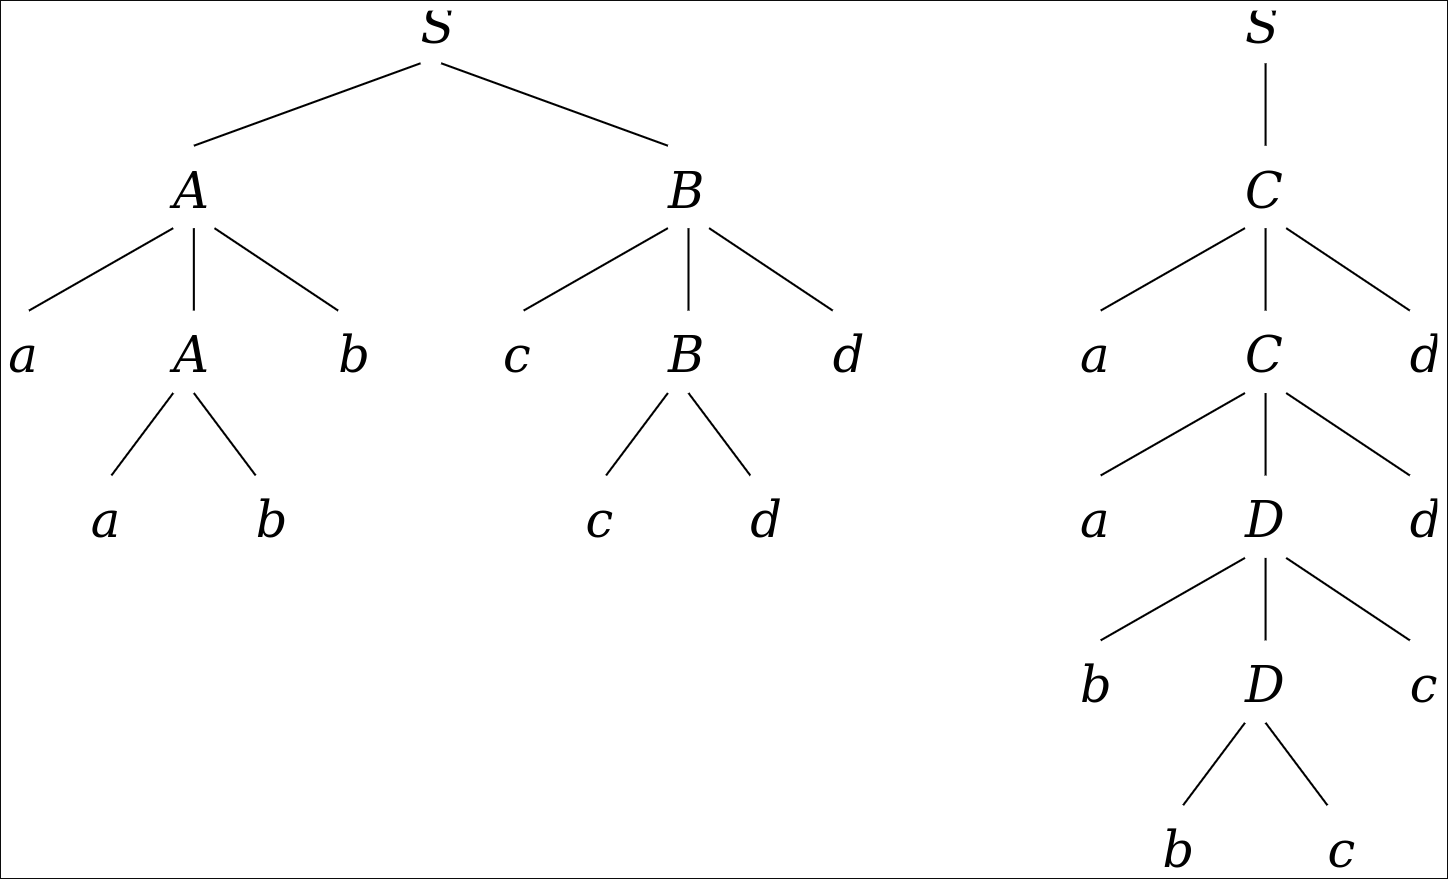
\includegraphics[width=.4\textwidth]{assets/20261015_162614.png}
    \end{cimage}
    \begin{note}
        Sono possibili due \hyperref[rem:gram-derivazione]{Derivazioni} a sinistra:
        \[
            S \underset{lm}{\implies}AB \underset{lm}{\implies}aAbB \underset{lm}{\implies}aabbB \underset{lm}{\implies}aaaabbcBd \underset{lm}{\implies}aabbccdd
        \]
        e
        \[
            S \underset{lm}{\implies}C \underset{lm}{\implies} aCd \underset{lm}{\implies}aaDdd \underset{lm}{\implies}aabDcdd \underset{lm}{\implies}aabbccdd
        \]
        \begin{warning}
            Può essere provato che ogni \hyperref[def:cfg]{Grammatica} per $L$ si comporta come questa, quindi il linguaggio $L$ è \hyperref[def:ambig-inerente]{Inerentemente Ambiguo}
        \end{warning}
    \end{note}
\end{example}
% subsection Ambiguità Inerente (end)
% section Ambiguità nelle Grammatiche e nei Linguaggi (end)
%
\section{Automi a Pila}\label{sec:ll_automi_a_pila} % (fold)
Un \textbf{automa a pila} è in sostanza un \hyperref[def:enfa]{Automa a Stati Finiti Non Deterministico con $\eps$-Transizioni} e una capacità aggiuntiva, ovvero uno \textbf{stack} in cui può memorizzare una stringa di simboli.
\begin{note}
    A differenza degli automi a stati finiti, grazie allo stack l'automa a pila può ricordare una quantità illimitata di informazioni
    \begin{warning}[Modalità di accesso LIFO]
    \end{warning}
\end{note}
Una transizione nell'automa a pila si può basare sullo stato corrente, sul simbolo di input e sul simbolo alla sommità dello stack; il tutto suddiviso in tre operazioni
\begin{enumerate}
    \item consuma il simbolo che usa nella transizione oppure in caso di $\eps$ non si consuma alcun simbolo;
    \item passa a un nuovo stato, che può essere o no uguale al precedente;
    \item sostituisce il simbolo in cima allo stack con una stringa che può essere:
        \begin{itemize}
            \item $\eps$ che corrisponde a togliere dallo stack;
            \item lo stesso simbolo che c'era prima alla sommità dello stack (lo stack non cambia);
            \item un altro simbolo che modifica la sommità dello stack (\red{senza inserire o rimuovere} valori dallo stack);
        \end{itemize}
\end{enumerate}
\begin{example}{}{}
    Consideriamo il linguaggio:
    \[
        L_{wwr} = \pg{ww^R : w\in\pg{0,1}^*}
    \]
    che corrisponde al linguaggio delle \hyperref[def:palindromo]{Palindrome} di lunghezza pari sull'alfabeto $\pg{0,1}$.
    È un \hyperref[chap:ll_linguaggi_liberi_dal_contesto]{Linguaggi Libero dal Contesto} generato dalla \hyperref[def:cfg]{Grammatica}:
    \[
        \begin{aligned}
            &P\to 0P0 \\
            &P\to 1P1 \\
            &P\to \eps \\
        \end{aligned}
    \]
    Un \hyperref[sec:pda]{PDA} per $L_{wwr}$ ha \textbf{tre stati}, e funziona come segue:
    \begin{enumerate}
        \item legge $w$ un simbolo alla volta, rimanendo nello stato $q_0$ aggiungendo i simboli alla pila;
        \item decide non deterministicamente che sta nel mezzo di $ww^R$ e va nello stato $q_1$;
        \item legge $w^R$ un simbolo alla volta e lo paragona con il simbolo in cima alla pila:
            \begin{itemize}
                \item se sono uguali, fa un pop della pila e rimane nello stato $q_1$;
                \item se sono diversi si blocca;
            \end{itemize}
        \item se la pila non ha più simboli ($0$ o $1$), va nello stato $q_2$ e accetta;
    \end{enumerate}
    \begin{cimage}
        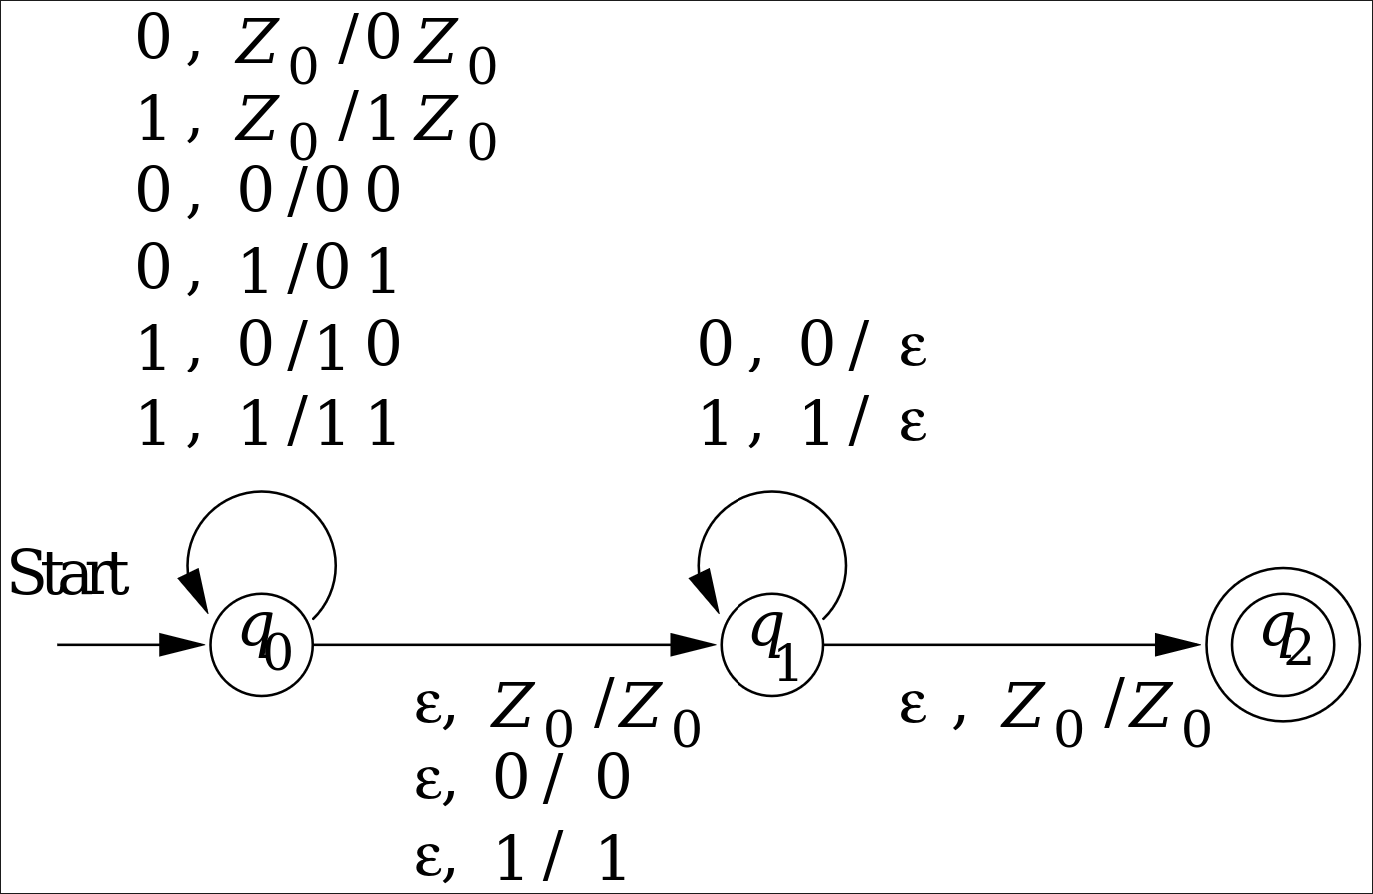
\includegraphics[width=.6\textwidth]{assets/20261022_152001.png}
        \caption{}\label{fig:20261022_152001}
    \end{cimage}
\end{example}
\begin{definition}{Automa a Pila}{pda}
    Un \textbf{PDA} è una tupla di $7$ elementi:
    \[
        P = (Q,\Si, \Gm, \dt, q_0, Z_0,F)
    \]
    dove:
    \begin{multicols}{2}
        \begin{itemize}
            \item $Q$ è un insieme finito di stati;
            \item $\Si$ è un alfabeto finito di input;
            \item $\Gm$ è un alfabeto finito di pila;
            \item $\dt$ è una funzione di transizione da $Q\times \pt{\Si \cup \pg \eps}\times \Gm$ a sottoinsiemi di $Q\times\Gm[*]$;
            \item $q_0$ è lo stato iniziale;
            \item $Z_0 \in $ è il simbolo iniziale per la pila;
            \item $F \subseteq Q$ è l'insieme di stati di accettazione;
        \end{itemize}
    \end{multicols}
\end{definition}
\begin{example}{}{}
    Il \hyperref[def:pda]{PDA} in \cref{fig:20261022_152001} è identificato dalla tupla:
    \[
        P = \pt{\pg{q_0,q_1,q_2}, \pg{0,1}, \pg{0,1,Z_0},\dt,q_0,Z_0,\pg{q_2}}
    \]
    dove $\dt$ è data dalla tabella:
    \begin{cimage}
        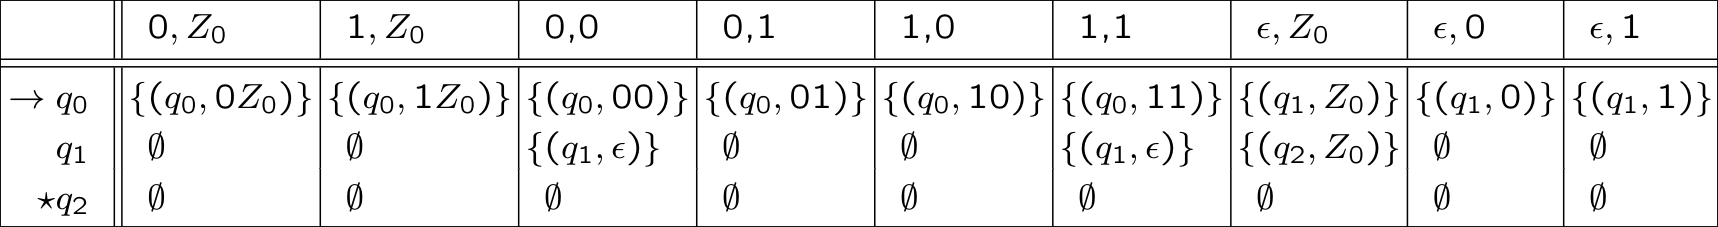
\includegraphics[width=\textwidth]{assets/20261022_154649.png}
    \end{cimage}
\end{example}
%
\subsection{Descrizioni Istantanee}\label{sub:ll_descrizioni_istantanee} % (fold)
Un \hyperref[def:pda]{Automa a Pila} passa da una configurazione a un'altra reagendo ai simboli di input (o $\eps$), ma diversamente dagli automi a stati finiti, la configurazione di un \hyperref[def:pda]{Automa a Pila} comprende sia lo \textbf{stato} sia il \textbf{contenuto dello stack}.
\emptyln{}
Di conseguenza una configurazione si rappresenta come una tripla $(q,w,\gm)$ dove:
\begin{itemize}
    \item $q$ è lo stato;
    \item $w$ è l'input residuo;
    \item $\gm$ è il contenuto dello stack;
\end{itemize}
\begin{definition}{Descrizione Istantanea}{desc-inst}
    La tripla $(q,w,\gm)$ viene chiamata \textbf{descrizione istantanea} (ID) dell'automa a pila.
\end{definition}
\begin{quote}
    Per gli automi a stati finiti la notazione $\hat\dt$ è sufficiente a rappresentare sequenze di descrizioni istantanee attraverso le quali un automa si muove (la \hyperref[def:desc-inst]{ID} coincide con lo stato)
\end{quote}
Per i \hyperref[def:pda]{PDA} occorre una notazione che descriva le trasformazioni di stato (input e stack).
Per connettere le coppie di \hyperref[def:desc-inst]{ID} che rappresentano una o più mosse di un \hyperref[def:pda]{Automa a Pila} si adotta la seguente notazione.
\begin{definition}{Chiusura PDA}{chiusura-pda}
    Sia $P = (Q,\Si, \Gm, \dt, q_0, Z_0,F)$ un \hyperref[def:pda]{Automa a Pila}.
    Supponiamo che $\dt\pt{q,\alpha,X}$ contenga $(p,\alpha)$, allora per tutte le stringhe $w$ in $\Si[*]$ e $\bt$ in $\Gm[*]$ definiamo $\underset{P}{\vdash}$, o $\vdash$ quando $P$ è sottinteso, come:
    \[
        \pt{q,\al w,X\bt} \vdash \pt{p,w,\al\bt}
    \]
    \begin{note}
        Si riflette l'idea che, consumando $\al$ dall'input e sostituendo $X$ alla sommità dello stack con $\al$, si può andare dallo stato $q$ allo stato $p$.
        \emptyln{}
        Inoltre quando rimane in input, $w$, e quando si trova sotto la cima dello stack, $\bt$, non influenza l'azione del \hyperref[def:pda]{PDA}, ma viene conservato e ha la possibilità di influenzare in seguito
    \end{note}
    Inoltre si utilizza il simbolo $\underset{P}{\vdash}^*$, o $\vdash^*$ quando $P$ è sottinteso, per rappresentare $0$ o più mosse del \hyperref[def:pda]{PDA}.
\end{definition}
\begin{example}{}{}
    Considerando l'azione del \hyperref[def:pda]{PDA} in \cref{fig:20261022_152001} su input $1111$, siccome $q_0$ è lo stato iniziale e $Z_0$ è il \textbf{simbolo iniziale}, la \hyperref[def:desc-inst]{ID} iniziale è $(q_0, 1111,Z_0)$.
    Su questo input il \hyperref[def:pda]{PDA} ha la possibilità di fare diverse congetture sbagliate.
    L'intera sequenza di \hyperref[def:desc-inst]{ID} che il \hyperref[def:pda]{PDA} può raggiungere dalla \hyperref[def:desc-inst]{ID} iniziale è rappresentata in \cref{fig:20261022_165743}.
    \begin{note}[Le frecce indicano la relazione $\vdash$]
    \end{note}
    \begin{cimage}
        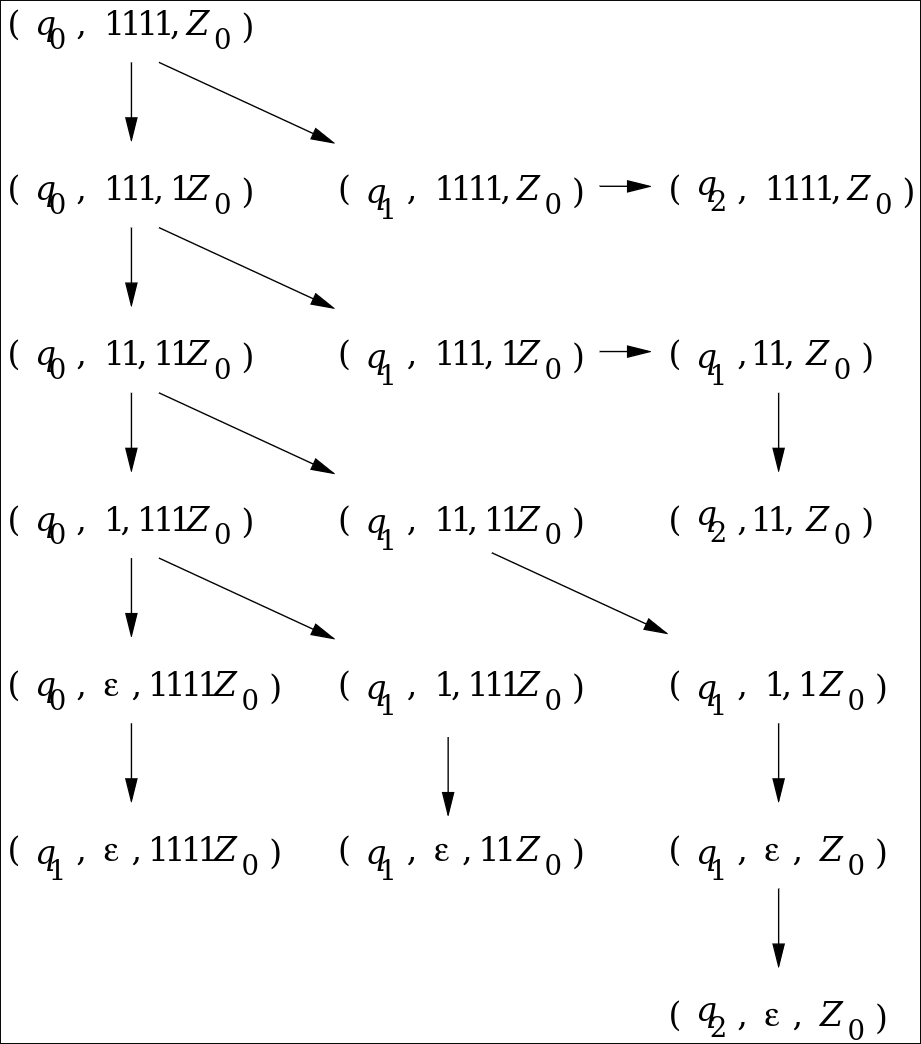
\includegraphics[width=.4\textwidth]{assets/20261022_165743.png}
        \caption{}\label{fig:20261022_165743}
    \end{cimage}
    A partire dalla \hyperref[def:desc-inst]{Descrizione Istantanea} iniziale ci sono due mosse possibili:
    \begin{itemize}
        \item la prima metà non sia stata vista e conduce alla \hyperref[def:desc-inst]{Descrizione Istantanea} $(q_0,111,1Z_0)$: un $1$ è stato rimosso dall'input e inserito nello stack;
        \item la prima metà sia stata raggiunta, quindi il \hyperref[def:pda]{PDA} va nello stato $q_1$ portando alla \hyperref[def:desc-inst]{Descrizione Istantanea} $(q_1, 1111,Z_0)$ senza consumo di input.
            Poiché accetta se si trova nello stato $q_1$ con $Z_0$ alla sommità dello stack, il \hyperref[def:pda]{PDA} passa alla \hyperref[def:desc-inst]{Descrizione Istantanea} $(q_2, 1111, Z_0)$, che non è accettante perché l'input non è stato interamente consumato.
    \end{itemize}
    \begin{note}
        Se l'input fosse stato $\eps$ invece di $1111$, la stessa sequenza di mosse avrebbe condotto alla \hyperref[def:desc-inst]{Descrizione Istantanea} $(q_2,\eps,Z_0)$ da cui sarebbe risultato chiaro che $\eps$ è accettata
    \end{note}
    Il \hyperref[def:pda]{PDA} può anche ipotizzare di aver visto la prima metà dopo aver letto un solo $1$, cioé quando si trova nella \hyperref[def:desc-inst]{Descrizione Istantanea} $(q_0,111,1Z_0)$.
    Dal momento che non si può consumare tutto l'input, anche questa scelta porta al fallimento.
    \emptyln{}
    La scelta corretta, cioè aver raggiunto la prima metà dopo aver letto $11$, fornisce la sequenza di \hyperref[def:desc-inst]{ID}:
    \[
        \begin{aligned}
            (q_0,1111,Z_0) &\vdash (q_0,111,1Z_0) \vdash (q_0,11,11Z_0) \vdash (q_1,11,11Z_0) \\
                           &\vdash (q_1,1,1Z_0) \vdash (q_1,\eps,Z_0) \vdash (q_2,\eps,Z_0)
        \end{aligned}
    \]
\end{example}
\begin{note}
    Nello studio dei \hyperref[def:pda]{PDA} hanno particolare importanza tre principi relativi alle \hyperref[def:desc-inst]{ID} e alle transizioni:
    \begin{itemize}
        \item se una sequenza di \hyperref[def:desc-inst]{ID}, chiamata \textbf{composizione}, è lecita per un \hyperref[def:pda]{PDA} $P$, allora è lecita anche la computazione formata accodando una stringa all'input in ogni \hyperref[def:desc-inst]{ID};
        \item se una computazione è lecita per un \hyperref[def:pda]{PDA} $P$, allora è lecita anche la computazione formata aggiungendo gli stessi simboli sotto quelli nello stack in ogni \hyperref[def:desc-inst]{ID};
        \item se una computazione è lecita per un \hyperref[def:pda]{PDA} $P$, e resta una coda di input non consumata, possiamo rimuovere il residuo dall'input in ogni \hyperref[def:desc-inst]{ID} e ottenere una computazione lecita;
    \end{itemize}
\end{note}
% subsection Descrizioni Istantanee (end)
%
\subsection{Accettazione per Stato Finale}\label{sub:ll_accettazione_per_stato_finale} % (fold)
Sia $P = (Q,\Si,\Gm,\dt,q_0,Z_0,F)$ un \hyperref[def:pda]{Automa a Pila}, allora $L(P)$, il \textbf{linguaggio accettato da $P$ per stato finale}, è:
\[
    \pg{w\,|\,\pt{q_0,w,Z_0} \underset{P}{\vdash}^* (q,\eps,\al)}
\]
per uno stato $q$ in $F$.
\begin{note}[In altre parole...]
    A partire dalla \hyperref[def:desc-inst]{Descrizione Istantanea} iniziale con $w$ in input, $P$ consuma $w$ ed entra in uno stato accettante.
    A questo punto il contenuto dello stack è irrilevante.
\end{note}
% subsection Accettazione per Stato Finale (end)
%
\subsection{Accettazione per Pila Vuota}\label{sub:ll_accettazione_per_pila_vuota} % (fold)
Per ogni \hyperref[def:pda]{PDA} $P = (Q,\Si,\Gm,\dt,q_0,Z_0,F)$ definiamo:
\[
    N(P) = \pg{w\,|\,(q_0,w,Z_0)\vdash* (q,\eps,\eps)}
\]
per qualsiasi stato $q$.
\begin{note}
    Quindi $N(P)$ è l'insieme degli input $w$ che $P$ può consumare, svuotando nel contempo lo stack
\end{note}
% subsection Accettazione per Pila Vuota (end)
%
\subsection{Da Stack Vuoto a Stato Finale}\label{sub:ll_da_stack_vuoto_a_stato_finale} % (fold)
\begin{theorem}{}{}
    Se $L = N(P_N)$ per un \hyperref[def:pda]{PDA} $P_N = (Q,\Si,\Gm,\dt_N,q_0,Z_0)$ allora esiste un \hyperref[def:pda]{PDA} $P_F$ tale che:
    \[
        L = L(P_F)
    \]
\end{theorem}
\begin{outerproof}{}
    Ci serviamo di un nuovo simbolo $X_0 \notin\Gm$ che rappresenta sia il simbolo iniziale di $P_F$ sia un segnale che indica quando $P_N$ ha svuotato lo stack.
    Quando $P_F$ vede $X_0$ alla sommità del proprio stack, sa che $P_N$ vuoterebbe lo stack sullo stesso input.
    \begin{cimage}
        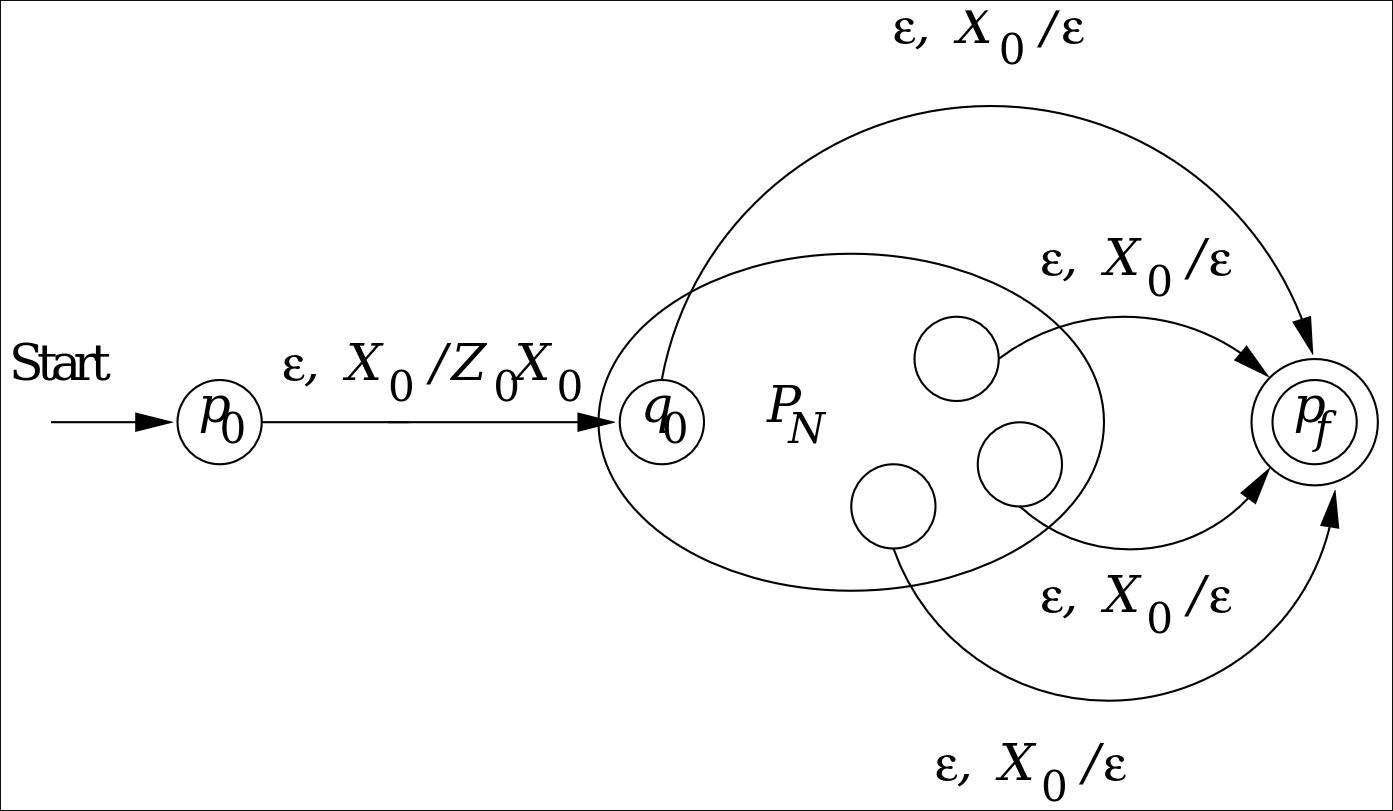
\includegraphics[width=.6\textwidth]{assets/20261022_183536.png}
    \end{cimage}
    Abbiamo inoltre bisogno di un nuovo stato iniziale $p_0$, la cui unica funzione è \red{inserire $Z_0$}, il simbolo iniziale di $P_N$, in cima allo stack ed entrare nello stato $q_0$, lo stato iniziale di $P_N$.
    \emptyln{}
    A questo punto $P_F$ simula $P_N$ finché lo stack di $P_N$ è vuoto: $P_F$ se ne accorge perché vede $X_0$ alla sommità dello stack.
    Infine occorre un altro nuovo stato $p_f$, che è lo stato accettante di $P_F$.
    \begin{note}
        Questo \hyperref[def:pda]{PDA} entra nello stato $p_f$ quando scopre che $P_N$ avrebbe svuotato il proprio stack
    \end{note}
    Quindi sia
    \[
        P_F = \pt{Q\cup\pg{p_0,p_f}, \Si,\Gm\cup\pg{X_0},\dt_F,p_0,X_0,\pg{p_f}}
    \]
    dove:
    \begin{itemize}
        \item $\dt_F\pt{p_0,\eps,X_0} = \pg{\pt{q_0,Z_0,X_0}}$, nel suo stato iniziale $P_F$ compie una transizione spontanea allo stato iniziale di $P_N$, inserendone il simbolo iniziale $Z_0$ sullo stack;
        \item per tutti gli stati $q \in Q$, gli input $a \in \Si\cup\pg\eps$, e i simboli di stack $Y \in\Gm$, $\dt_F\pt{q,a,Y}$ contiene tutte le coppie in $\dt_N\pt{q,a,Y}$;
        \item $\dt_F\pt{q,\eps,X_0}$ contiene $(p_f,\eps)$ per ogni stato $q\in Q$;
    \end{itemize}
\end{outerproof}
\begin{example}{}{}
    Il seguente \hyperref[def:pda]{PDA} elabora sequenze di \texttt{if} e \texttt{else} in un programma dove $i$ sta per \texttt{if} e $e$ sta per \texttt{else}.
    \begin{warning}
        C'è un problema ogni volta che il numero di \texttt{else} in un prefisso eccede il numero di \texttt{if}, perché in quel caso non si possono abbinare ogni \texttt{else} al \texttt{if} che lo precede.
        \begin{tip}
            Si utilizza il simbolo di stack $Z$ per contare la differenza tra il numero di $i$ e il numero di $e$ letti
        \end{tip}
    \end{warning}
    \begin{cimage}
        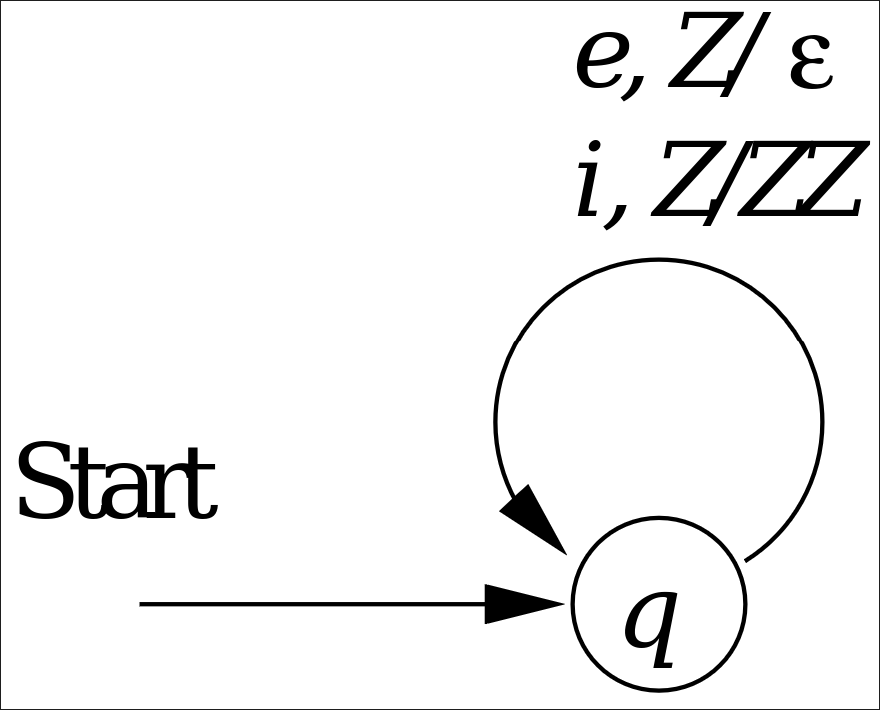
\includegraphics[width=.2\textwidth]{assets/20261022_192132.png}
        \caption{}\label{fig:20261022_192132}
    \end{cimage}
    Inseriamo una $Z$ quando leggiamo una $i$ e la eliminiamo quando leggiamo una $e$.
    Poiché partiamo con una $Z$ nello stack, allora il numero di $i$ letti supera quello degli $e$ e di $\dec n$.
    \begin{note}
        In particolare lo stack è vuoto se abbiamo letto una $e$ in più rispetto alle $i$, e l'input letto fino a questo punto è diventato illecito per la prima volta
    \end{note}
    Formalmente $P_N$ può essere scritto come:
    \[
        P_N = \pt{\pg q, \pg{i,e}, \pg Z,\dt_N,q,Z}
    \]
    dove $\dt_N$ è definita come:
    \begin{itemize}
        \item $\dt_N\pt{q,i,Z} = \pg{\pt{q,ZZ}}$, inserisce una $Z$ quando leggiamo una $i$;
        \item $\dt_N\pt{q,e,Z} = \pg{\pt{q,\eps}}$, elimina una $Z$ quando leggiamo una $e$;
    \end{itemize}
    \begin{note}
        A partire da $P_N$ si costruisce un \hyperref[def:pda]{PDA} $P_F$ che accetta lo stesso linguaggio, \textbf{ma} \hyperref[sub:ll_accettazione_per_stato_finale]{Stato Finale}
    \end{note}
    Viene introdotto un nuovo stato iniziale $p$ e uno accettante $r$, usando $X_0$ come segnale di fondo dello stack.
    Formalmente si definisce:
    \[
        P_F = \pt{\pg{p,q,r},\pg{i,e},\pg{Z,X_0},\dt_F,p,X_0,\pg r}
    \]
    dove $\dt_F$ consiste delle seguenti regole:
    \begin{itemize}
        \item $\dt_F\pt{q,\eps,X_0} = \pg{\pt{q,ZX_0}}$, fa partire $P_F$ simulando $P_N$ con $X_0$ come indicatore di fondo dello stack;
        \item $\dt_F\pt{q,i,Z} = \pg{\pt{q,ZZ}}$, inserisce una $Z$ quando leggiamo una $i$;
        \item $\dt_F\pt{q,e,Z} = \pg{\pt{q,\eps}}$, elimina una $Z$ quando leggiamo una $e$;
        \item $\dt_F\pt{q,\eps,X_0} = \pg{\pt{r,\eps}}$, $P_F$ accetta nei casi in cui $P_N$ svuota il proprio stack;
    \end{itemize}
    Il diagramma per $P_F$ è il seguente:
    \begin{cimage}
            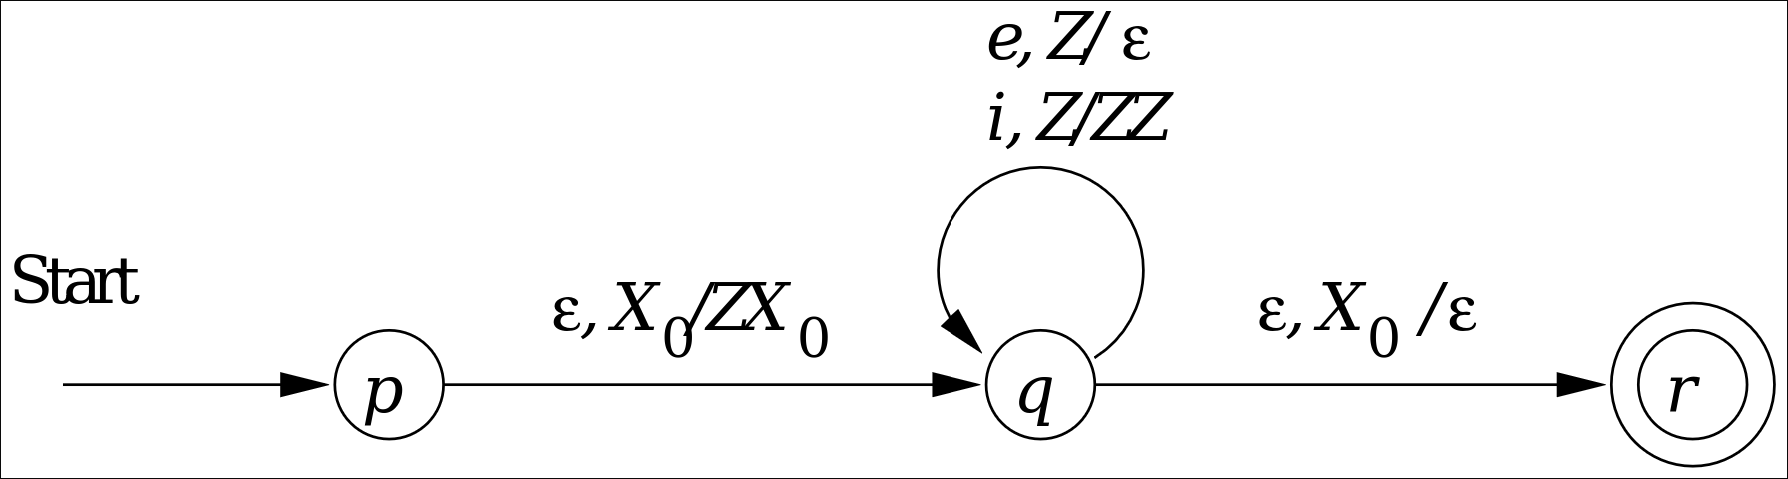
\includegraphics[width=.6\textwidth]{assets/20261022_194714.png}
    \end{cimage}
\end{example}
% subsection Da Stack Vuoto a Stato Finale (end)
%
\subsection{Da Stato Finale a Stack Vuoto}\label{sub:ll_da_stato_finale_a_stack_vuoto} % (fold)
\begin{theorem}{}{}
    Sia $L=L(P_F)$ per un \hyperref[def:pda]{PDA} $P_F = (Q,\Si,\Gm,\dt_F,q_0,Z_0,F)$, allora esiste un \hyperref[def:pda]{PDA} tale che:
    \[
        L = N(P_N)
    \]
\end{theorem}
\begin{outerproof}{}{}
    \begin{cimage}
        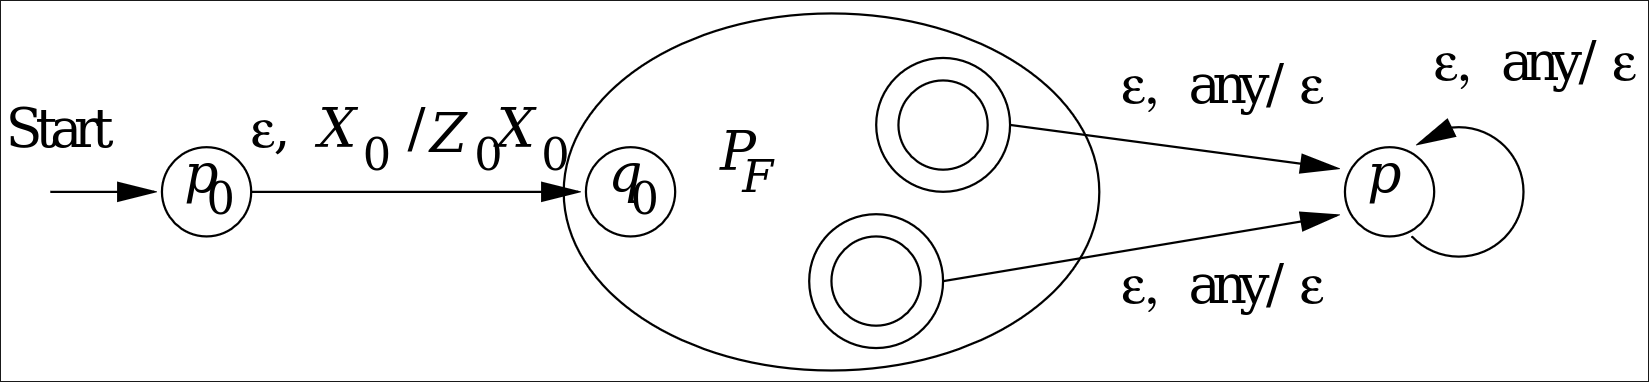
\includegraphics[width=.8\textwidth]{assets/20261022_200043.png}
        \caption{}\label{fig:20261022_200043}
    \end{cimage}
    La costruzione è quella seguita in \cref{fig:20261022_200043}, sia:
    \[
        P_N = \pt{Q\cup \pg{p_0,p},\Si,\Gm\cup \pg{X_0},\dt_N,p_0,X_0}
    \]
    dove $\dt_N$ è definita come:
    \begin{itemize}
        \item $\dt_N \pt{p_0,\eps,X_0} = \pg{\pt{q_0,Z_0,X_0}}$, si inserisce il simbolo iniziale di $P_F$ nello stack e andando nello stato iniziale di $P_F$;
        \item per ogni stato $q\in Q$, ogni simbolo di input $a\in\Si\cup \pg{\eps}$ e ogni $Y\in\Gm$, $\dt_N \pt{q,a,Y}$;
            \begin{note}
                In altre parole $P_N$ simula $P_F$
            \end{note}
        \item per tutti gli stati accettanti in $q\in F$ e i simboli di stack $Y\in \Gm\cup \pg{X_0}$, $\dt_N \pt{q,\eps,Y}$ contiene $\pt{p,\eps}$;
            \begin{note}
                Per questa regola, ogni volta che $P_F$ accetta $P_N$ può cominciare a vuotare il suo stack senza consumare ulteriori input
            \end{note}
        \item per tutti i simboli di stack $Y \in \Gm \cup \pg{X_0}$, $\dt_N \pt{p,\eps,Y} = \pg{\pt{p,\eps}}$;
            Giunto nello stato $p$, il che è possibile solo quando $P_F$ ha accettato, $P_N$ elimina ogni simbolo nel suo stack fino a vuotarlo (senza consumare altri input).
    \end{itemize}
\end{outerproof}
% subsection Da Stato Finale a Stack Vuoto (end)
% section Automi a Pila (end)
%
\section{Equivalenza di PDA e CFG}\label{sec:ll_equivalenza_di_pda_e_cfg} % (fold)
\begin{remark}{}{}
    Un \hyperref[def:linguaggio]{Linguaggio} è generato da una \hyperref[def:cfg]{Grammatica Libera dal Contesto} \textbf{se e solo se} è accettato da un \hyperref[def:pda]{Automa a Pila} per \hyperref[sub:ll_accettazione_per_pila_vuota]{Pila Vuota} \textbf{se e solo se} è accettato da un \hyperref[def:pda]{Automa a Pila} per \hyperref[sub:ll_accettazione_per_stato_finale]{Stato Finale}
\end{remark}
\begin{cimage}
    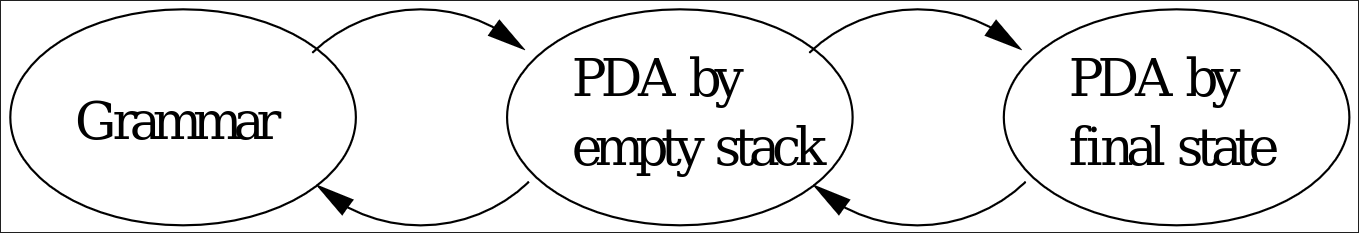
\includegraphics[width=.8\textwidth]{assets/20261022_201732.png}
\end{cimage}
%
\subsection{Dalle Grammatiche agli Automi a Pila}\label{sub:ll_dalle_grammatiche_agli_automi_a_pila} % (fold)
Data una \hyperref[sec:ll_grammatiche_libere_dal_contesto]{Grammatica Libera dal Contesto} $G$, si costruisce un \hyperref[def:pda]{PDA} che ne simula la derivazione a sinistra $\pt{\overset{*}{\underset{lm}{\implies}}}$.
\\
Ogni forma sentenziale sinistra, che non sia una stringa terminale, si può scrivere nella forma:
\[
    xA\al
\]
dove $A$ è la variabile \textbf{più a sinistra}, $x$ è la stringa di terminali alla sua sinistra, e $\al$ è la stringa di terminali e variabili alla destra di $A$.
\begin{example}{}{}
    \[
        \underbrace{(\al + }_{x}\underbrace{\underbrace{E}_{A}\underbrace{)}_{\al}}_{tali}
    \]
\end{example}
\begin{tip}
    La costruzione di un \hyperref[def:pda]{Automa a Pila} da una \hyperref[def:cfg]{Grammatica} poggia sull'idea di far simulare al \hyperref[def:pda]{PDA} la serie di \textbf{forme sentenziali sinistre} usate dalla \hyperref[def:cfg]{Grammatica} per generare una stringa terminale data $w$
\end{tip}
La coda di ogni forma $xA\al$ compare sullo stack con $A$ in cima.
In quel momento $x$ è rappresentata dall'aver consumato $x$ in input, lasciando ciò che in $w$ segue $x$.
\begin{note}[Quindi se $w = xy$ allora in input rimane $y$]
\end{note}
\begin{remark}{}{}
    Supponiamo che il \hyperref[def:pda]{PDA} si trovi nella \hyperref[def:desc-inst]{ID} $(q,y,A\al)$, che rappresenta la forma sentenziale sinistra $xA\al$, l'automa sceglie arbitrariamente una produzione per espandere $A$.
    Poniamo $A\to \bt$, la sua mossa consiste nel sostituire $A$ con $\bt$ in cima allo stack, entrando nella \hyperref[def:desc-inst]{ID} $(q,y,\bt\al)$.
    \begin{note}
        Il \hyperref[def:pda]{PDA} ha un solo stato $q$
    \end{note}
    La \hyperref[def:desc-inst]{Descrizione Istantanea} $(q,y,\bt\al)$ potrebbe non rappresentare la successiva forma sentenziale sinistra, perché $\bt$ può avere un prefisso formato da \textbf{terminali}.
    Di fatto può darsi che $\bt$ non contenga affatto variabili e che $\al$ abbia un prefisso composto di \textbf{terminali}.
    \emptyln{}
    Per esporre in cima allo stack la prossima variabile, dobbiamo eliminare gli eventuali terminali all'inizio di $\bt\al$.
    Questi terminali vanno confrontati con i successivi simboli di input per verificare che le scelte per \hyperref[rem:gram-derivazione]{Derivazione} a sinistra della stringa di input $w$ siano corrette; in caso contrario la diramazione del \hyperref[def:pda]{PDA} muore.
\end{remark}
Se in questo modo si determina una \hyperref[rem:gram-derivazione]{Derivazione} a sinistra di $w$, alla fine si raggiunge la forma sentenziale sinistra $w$.
A quel punto ogni simbolo sullo stack o è stato espanso (\red{caso delle variabili}) o abbinato a un simbolo di input (\red{caso dei terminali}), quindi lo \textbf{stack è vuoto} e \textbf{l'automa accetta}.  
\emptyln{}
A questo punto è possibile definire la seguente costruzione: sia $G = (V,T,Q,S)$ una \hyperref[def:cfg]{Grammatica Libera dal Contesto}, costruiamo il \hyperref[def:pda]{PDA} $P$ che accetta $L(G)$ per stack vuoto:
\[
    P = \pt{\pg{q},T,V\cup T,\dt,q,S}
\]
La funzione di transizione $\dt$ è definita come:
\begin{itemize}
    \item per ogni variabile $A$:
        \[
            \dt \pt{q,\eps,A} = \pg{\pt{q,\bt}\,|\, A\to\bt\text{ è una produzione di }G}
        \]
    \item per ogni terminale $a$, $\dt \pt{q,a,a} = \pg{\pt{q,\eps}}$
\end{itemize}
\begin{example}{}{}
    Considerando l'alfabeto $\pg{i,e}$ e la seguente grammatica:
    \[
        S \to\eps|SS|iS|iSe
    \]
    Determiniamo la funzione di transizione:
    \begin{itemize}
        \item $\dt \pt{q,\eps,S} = \pg{\pt{q,\eps}, \pt{q,SS}, \pt{q,iS}, \pt{q,iSe}}$
        \item $\dt \pt{q,i,i} = \pg{\pt{q,\eps}}$
        \item $\dt \pt{q,e,e} = \pg{\pt{q,e}}$
    \end{itemize}
    Quindi il \hyperref[def:pda]{PDA} corrispondente si può esprimere come:
    \[
        P = \pt{\pg{q}, \pg{i,e}, \pg{S,i,e}, \dt, q, S}
    \]
    \begin{flushright}
        \qedsymbol
    \end{flushright}
\end{example}
% subsection Dalle Grammatiche agli Automi a Pila (end)
%
\subsection{Da Automa a Pila a Grammatica}\label{sub:ll_da_automa_a_pila_a_grammatica} % (fold)

% subsection Da Automa a Pila a Grammatica (end)
% section Equivalenza di PDA e CFG (end)
% chapter Linguaggi Liberi dal Contesto(end)
